% 2012_syllabus_science_q18_fig1: schematic quadrangular pyramid P-ABCD, E on PC
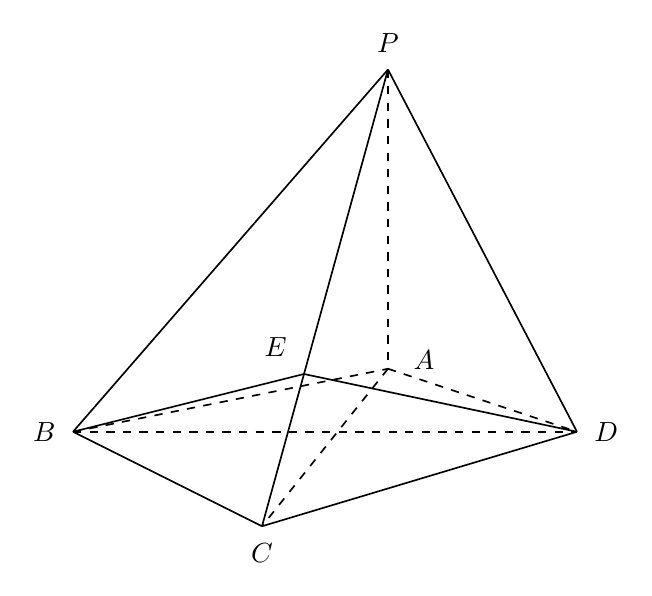
\begin{tikzpicture}[x=1cm,y=1cm,font=\normalsize,line width=.6pt]
\coordinate (P) at (0.6000000000,5.2000000000);
\coordinate (A) at (0.6,1.4);
\coordinate (B) at (-3.4,0.6);
\coordinate (C) at (-1.0,-0.6);
\coordinate (D) at (3.0,0.6);
\coordinate (E) at (-0.4666666667,1.3333333333);
% solid visible edges
\draw[solid] (P) -- (B);
\draw[solid] (P) -- (E);
\draw[solid] (E) -- (C);
\draw[solid] (P) -- (D);
\draw[solid] (B) -- (C);
\draw[solid] (C) -- (D);
\draw[solid] (B) -- (E);
% hidden edges
\draw[dashed] (P) -- (A);
\draw[dashed] (B) -- (A);
\draw[dashed] (A) -- (D);
\draw[dashed] (A) -- (C);
\draw[dashed] (B) -- (D);
\draw[solid] (E)--(D);
% labels with clearance
\node[inner sep=2pt,above=4pt] at (P) {$P$};
\node[inner sep=2pt,left=4pt] at (B) {$B$};
\node[inner sep=2pt,below=4pt] at (C) {$C$};
\node[inner sep=2pt,right=4pt] at (D) {$D$};
\node[inner sep=2pt,above left=4pt] at (E) {$E$};
\node[inner sep=2pt,right=4pt,xshift=3pt,yshift=3pt] at (A) {$A$};
\end{tikzpicture}
